% !TEX root = ./notes.tex
\documentclass[11pt,twoside]{book}
\usepackage[mono=false]{libertine} % new linux font, ignore mono

% avoid bugs with xy-pic, luatex, pdftex version
% \input{luatex-pdf}
\usepackage{luatex85}
% \usepackage[all]{xy}

%\renewcommand{\baselinestretch}{1.05}
\usepackage{amsmath,amsthm,amssymb,mathrsfs,amsfonts,dsfont}
\usepackage{epsfig,graphicx}
\usepackage{tabularx}
\usepackage{blkarray}
\usepackage{slashed}
\usepackage{color}
\usepackage{listings}
\usepackage{caption}
% \usepackage{fullpage}
\usepackage[toc,title,titletoc,header]{appendix}
\usepackage{color}
\usepackage{dcolumn}
\usepackage{bm}
\usepackage{hyperref}
\hypersetup{
    %citecolor=black,
    colorlinks=true,
    % linkcolor=blue,
    filecolor=magenta,      
    urlcolor=cyan,
}
\usepackage[capitalise]{cleveref}
\usepackage{subcaption}
\usepackage{enumitem}
\usepackage{mathtools}
\usepackage{braket}
\usepackage{cancel}
\usepackage{physics}
\usepackage{qcircuit}
\usepackage{tikz}
\usepackage{simpler-wick}
\usepackage[compat=1.1.0]{tikz-feynman}
\usepackage{braids}
\usepackage[linesnumbered,ruled,vlined,algosection]{algorithm2e}
\SetCommentSty{textsf}
% \usepackage{epigraph}
% \epigraphwidth=0.9\linewidth

\topmargin-1.2cm
% \headheight0.0cm
\headheight13.6pt
\headsep1.2cm
\oddsidemargin0.0cm
\evensidemargin0.0cm
\textheight23.0cm
\textwidth16.9cm
\footskip1.0cm

\usepackage{thmtools}
\declaretheorem[numberwithin=chapter]{theorem}
\declaretheorem[numberwithin=chapter]{axiom}
\declaretheorem[numberwithin=chapter]{lemma}
\declaretheorem[numberwithin=chapter]{proposition}
\declaretheorem[numberwithin=chapter]{claim}
\declaretheorem[numberwithin=chapter]{conjecture}
\declaretheorem[sibling=theorem]{corollary}
\declaretheorem[numberwithin=chapter, style=definition]{definition}
\declaretheorem[numberwithin=chapter, style=definition]{problem}
\declaretheorem[numberwithin=chapter, style=definition]{example}
\declaretheorem[numberwithin=chapter, style=definition]{exercise}
\declaretheorem[numberwithin=chapter, style=definition]{observation}
\declaretheorem[numberwithin=chapter, style=definition]{fact}
\declaretheorem[numberwithin=chapter, style=definition]{construction}
\declaretheorem[numberwithin=chapter, style=definition]{remark}
\declaretheorem[numberwithin=chapter, style=remark]{question}

% \theoremstyle{plain}
% \newtheorem{theorem}{Theorem}[chapter]
% \newtheorem{remark}{Remark}[chapter]
% \newtheorem{claim}{Claim}[chapter]
% \newtheorem{corollary}{Corollary}[theorem]
% \newtheorem{lemma}{Lemma}[chapter]
% \newtheorem{question}{Question}[chapter]
% \newtheorem{proposition}{Proposition}[chapter]
% \newtheorem{conjecture}{Conjecture}[chapter]
% \theoremstyle{definition}
% \newtheorem{example}{Example}[chapter]
% \newtheorem{exercise}{Exercise}[chapter]
% \newtheorem{definition}{Definition}[chapter]
% \newtheorem{observation}{Observation}[chapter]
% \newtheorem{fact}{Fact}[chapter]
% \newtheorem{construction}{Construction}[chapter]

\newenvironment{solution}
    {\renewcommand\qedsymbol{$\square$}\color{blue}\begin{adjustwidth}{0em}{2em}\begin{proof}[\textit Solution.~]}
    {\end{proof}\end{adjustwidth}}

\usepackage{makeidx}
\usepackage[nottoc]{tocbibind}
% \renewcommand{\index}[1]{\index{#1} \emph{#1}}
\newcommand{\myindex}[1]{\index{#1} \emph{#1}}
\makeindex
\usepackage[totoc]{idxlayout} % add index to toc

\usepackage{fancyhdr}
\pagestyle{fancy} % enable fancy page style
\renewcommand{\headrulewidth}{0.0pt} % comment if you want the rule
\fancyhf{} % clear header and footer
\fancyhead[re]{\slshape\nouppercase{\leftmark}}
\fancyhead[lo]{\slshape\nouppercase{\rightmark}}
\fancyhead[ro,le]{\thepage} % page number left(odd), right(even)

% \usepackage[numbers]{natbib}
% \bibliographystyle{plainnat} 


\usepackage[doi=false,url=false,isbn=false,style=alphabetic,backend=biber]{biblatex}
\addbibresource{bib.bib}

\newbibmacro{string+doiurlisbn}[1]{%
  \iffieldundef{doi}{%
    \iffieldundef{url}{%
      \iffieldundef{isbn}{%
        \iffieldundef{issn}{%
          #1%
        }{%
          \href{http://books.google.com/books?vid=ISSN\thefield{issn}}{#1}%
        }%
      }{%
        \href{http://books.google.com/books?vid=ISBN\thefield{isbn}}{#1}%
      }%
    }{%
      \href{\thefield{url}}{#1}%
    }%
  }{%
    \href{http://dx.doi.org/\thefield{doi}}{#1}%
  }%
}

% \DeclareFieldFormat{title}{\usebibmacro{string+doiurlisbn}{#1}}
% \DeclareFieldFormat[article,incollection]{title}{\usebibmacro{string+doiurlisbn}{\mkbibquote{#1}}}

% https://tex.stackexchange.com/questions/94089/remove-quotes-from-inbook-reference-title-with-biblatex
\DeclareFieldFormat[article,incollection,inproceedings,book,misc]{title}{\usebibmacro{string+doiurlisbn}{\mkbibemph{#1}}}
% https://tex.stackexchange.com/questions/454672/biblatex-journal-name-non-italic
\DeclareFieldFormat{journaltitle}{#1\isdot}
\DeclareFieldFormat{booktitle}{#1\isdot}
% https://tex.stackexchange.com/questions/10682/suppress-in-biblatex
\renewbibmacro{in:}{}

% \renewbibmacro{arxiv:}{}
% https://tex.stackexchange.com/questions/367197/shorten-biblatex-output
% \DeclareFieldFormat{eprint:arxiv}{%
% %  arXiv\addcolon\space
%   \ifhyperref
%     {\href{http://arxiv.org/\abx@arxivpath/#1}{%
%        \nolinkurl{#1}%
%        \iffieldundef{eprintclass}
%          {}
%          {\addspace\texttt{\mkbibbrackets{\thefield{eprintclass}}}}}}
%     {\nolinkurl{#1}
%      \iffieldundef{eprintclass}
%        {}
%        {\addspace\texttt{\mkbibbrackets{\thefield{eprintclass}}}}}}

% !TEX root = ./notes.tex
\usepackage[style=super]{glossaries}
\setlength{\glsdescwidth}{1\linewidth}
\makeglossaries

\renewcommand\glossaryname{List of Abbreviations and Symbols}

\newglossaryentry{Q2}{name={$Q_2(f)$},
%sort=Q2,
description={Two-side (bounded) error quantum query complexity}}
\newglossaryentry{real_number}{name={$\mathbb{R}$},description={Real number}}
% !TEX root = ./notes.tex

%%%%%%%%%%%%%%%%%%%%%%%%%%%%%%%%%%%%
%%%%%%%%%%%%%%%%%%%%%%%%%%%%%%%%%%%%
% math
\let\iff\relax
\newcommand{\iff}{\text{ iff }}
\newcommand{\OPT}{\textup{OPT}}

% physics
\newcommand{\acreation}{a^\dagger}



\begin{document}

\title{\bf \huge Study Notes}
\author{Author}
\maketitle
\setcounter{tocdepth}{2}

\tableofcontents
\listoffigures
% \listoftables
\listoftheorems[ignoreall,show={theorem}]
\renewcommand{\listtheoremname}{List of Definitions}
\listoftheorems[ignoreall,show={definition}]

\printglossaries

%%%%%%%%%%%%%%%Content%%%%%%%%%%%%%%%
% \mainmatter % separat the number of toc and mainmatter
% !TEX root = ../notes_template.tex
\chapter{Preface}

\section{Features of this template}

\begin{itemize}
    \item different styles of clickable definitions and theorems
    \begin{itemize}
        \item nameref:
            \nameref{def:gaussian_distribution}

        \item autoref:
            \autoref{def:gaussian_distribution}

        \item cref:
            \cref{def:gaussian_distribution}

        \item hyperref:
            \hyperref[def:gaussian_distribution]{Gaussian}
    \end{itemize}

    \item toc: list of theorems, definitions
    \item bib: titles of reference is linked to the publisher webpage 
        \cite{kitaev2002classical}
        \cite{childsUniversalComputationQuantum2009}
    \item index
    \myindex{index} 
    \item glossary
    \gls{real_number}
\end{itemize}

\begin{figure}[!ht]
    \centering
    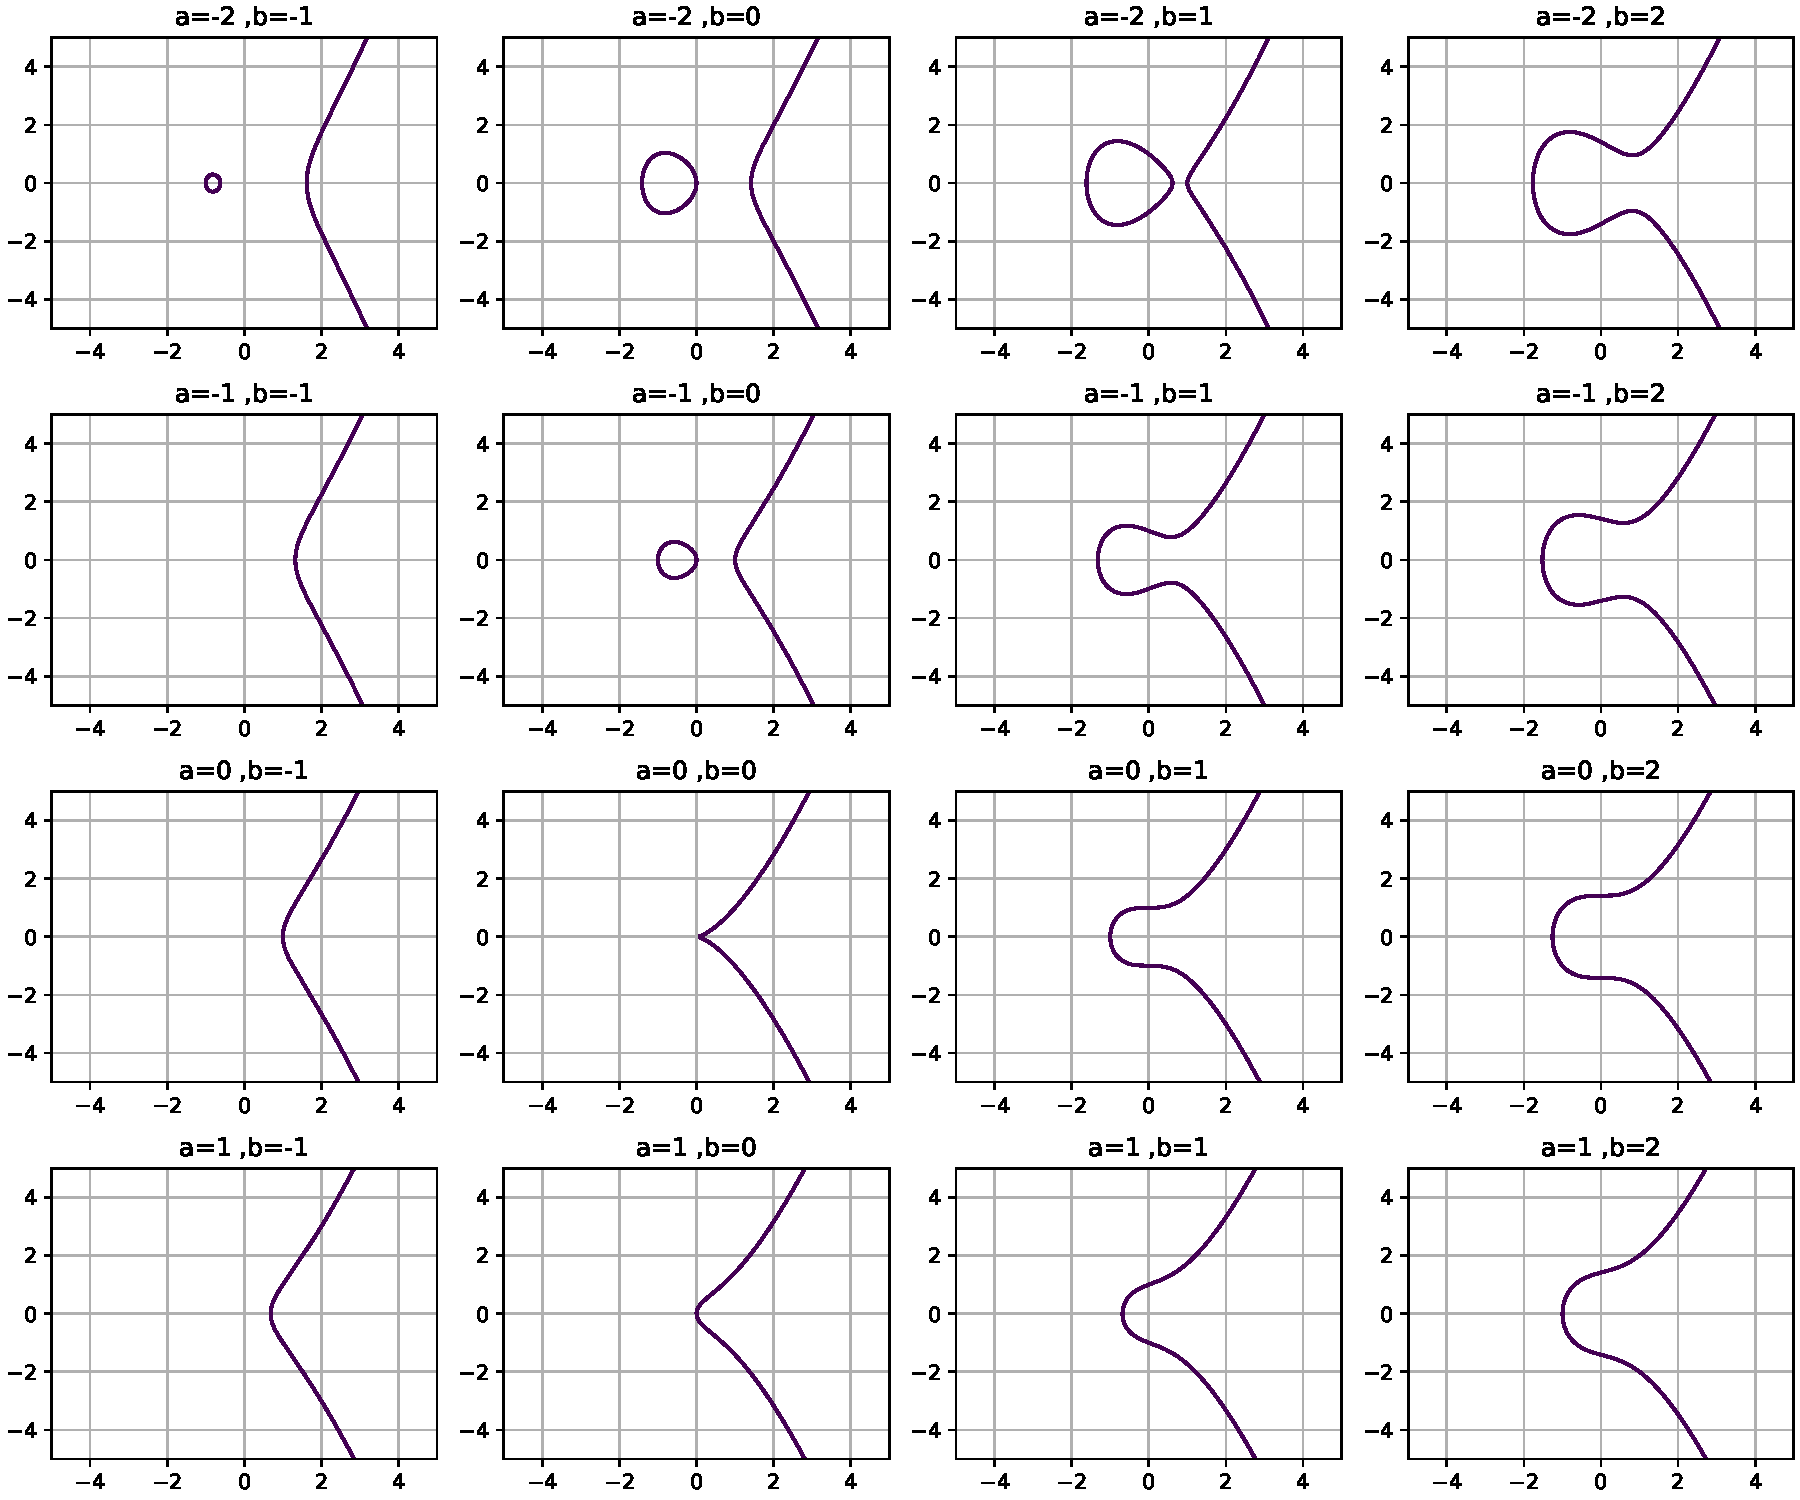
\includegraphics[width=1\linewidth]{./figure/elliptic_curves.pdf}
    \caption{Elliptic curves}
\end{figure}


\part{Mathematics}
% !TEX root = ../notes_template.tex
\chapter{Discrete Math}\label{chp:discrete_math}

\minitoc

gls examples:
\begin{itemize}
	% \item \glsxtrshort{gcd};
	\item \Gls{gcd}; \acrlong{gcd}; \acrshort{gcd}; \acrfull{gcd}
\end{itemize}

\section{Proof}
\begin{lemma}
\end{lemma}
\begin{claim}
\end{claim}
\begin{theorem}
\end{theorem}
\begin{example}
\end{example}
\begin{fact}
\end{fact}
\begin{remark}
\end{remark}
\begin{exercise}
	Prove A \iff B
\end{exercise}
\begin{solution}
By induction:
\end{solution}

\lipsum % dummy text - remove from real document

\section{Quantifier}
\lipsum % dummy text - remove from real document

\section{Graph}
\citetitle{babaiGraphIsomorphismQuasipolynomial2016}
\cite{babaiGraphIsomorphismQuasipolynomial2016}

\section{Number theory}
a Figure example
\begin{figure}[!ht]
    \centering
    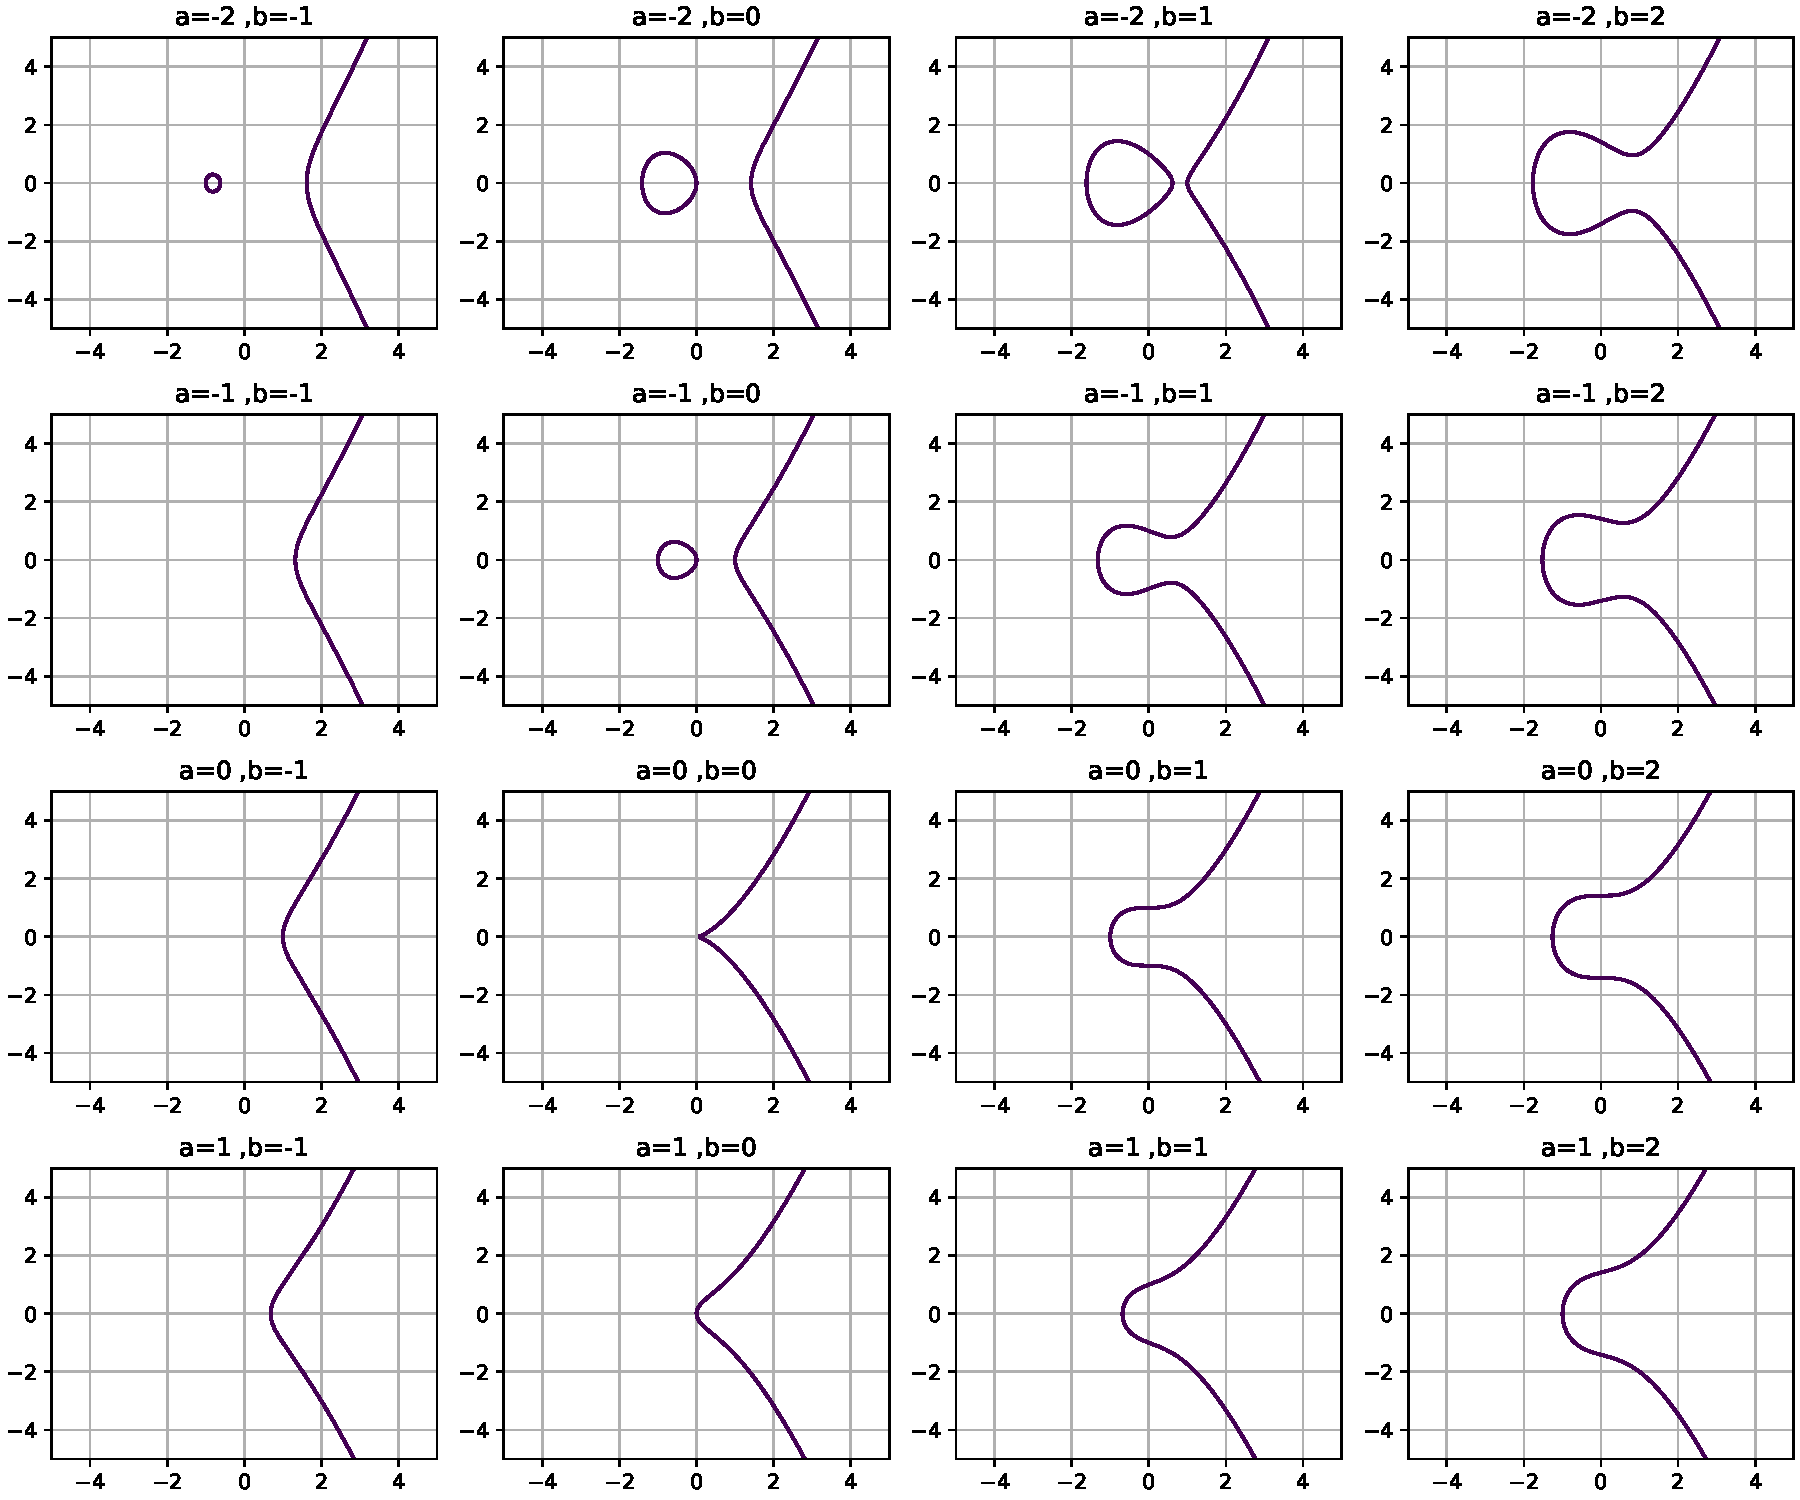
\includegraphics[width=1\linewidth]{./figure/elliptic_curves.pdf}
    \caption{Elliptic curves \cite{childsUniversalComputationQuantum2009} }
\end{figure}


\section{Algorithm}
% \begin{center}
% \begin{minipage}{.9\linewidth}
% algorithm2e
% https://www.overleaf.com/learn/latex/Algorithms#The_algorithm2e_package
\begin{algorithm}[H]
    \SetKwInOut{Input}{input}
    \SetKwInOut{Output}{output}
    \Input{Integer $N$ and parameter $1^t$}
    \Output{A decision as to whether $N$ is prime or composite}
    \BlankLine
    \For{ $i = 1,2, \ldots, t$} {
        $a\leftarrow \qty{1,\dots,N_1}$\;
        \If{$a^{N-1} \neq 1 \mod{N}$}
    {\Return "composite"}
    }
    \Return "prime"
    \caption{Primality testing - first attempt}
    \label{alg:miller_rabin}
\end{algorithm}
% \end{minipage}
% \end{center}

\part{Computer Science}
% \input{./chapter/algorithms.tex}


\part{Physics}
% \input{./chapter/quantum_field_theory.tex}

\begin{appendices}
% !TEX root = ../notes_template.tex
\chapter{Formulas}

\section{Gaussian distribution}\label{sec:gaussian_distribution}
\begin{definition}[Gaussian distribution]\label{def:gaussian_distribution}
    \myindex{Gaussian distribution}
\end{definition}

\begin{theorem}[Central limit theorem]\label{thm:central_limit_theorem}
\end{theorem}
\end{appendices}

\backmatter

%%%%%%%%%%%%%%% Reference %%%%%%%%%%%%%%%

\printbibliography
\printindex

\end{document}
